\documentclass[conference]{IEEEtran}
\IEEEoverridecommandlockouts

% ---------- Paquetes ----------
\usepackage{cite}
\usepackage{amsmath,amssymb,amsfonts}
\usepackage{algorithmic}
\usepackage{graphicx}
\usepackage{textcomp}
\usepackage{xcolor}
\usepackage{booktabs}
\usepackage{array}
\usepackage{listings}
\usepackage[spanish]{babel}
\usepackage[utf8]{inputenc}
\usepackage[T1]{fontenc}
\usepackage{hyperref}

% ---------- Estilo de listings para SystemVerilog ----------
\definecolor{svgreen}{rgb}{0,0.5,0}
\definecolor{svgray}{rgb}{0.5,0.5,0.5}
\definecolor{svblue}{rgb}{0,0,0.7}
\definecolor{svpurple}{rgb}{0.58,0,0.82}

\lstdefinelanguage{SystemVerilog}{
  morekeywords={class,extends,function,endfunction,task,endtask,virtual,
    begin,end,if,else,for,foreach,case,endcase,default,rand,constraint,
    dist,inside,logic,bit,int,unsigned,byte,void,super,new,this,return,
    typedef,enum,localparam,protected,local,forever,packed,string},
  morecomment=[l]{//},
  morecomment=[s]{/*}{*/},
  morestring=[b]",
}

\lstdefinestyle{sv}{
  language=SystemVerilog,
  basicstyle=\scriptsize\ttfamily,
  keywordstyle=\color{svblue}\bfseries,
  commentstyle=\color{svgreen}\itshape,
  stringstyle=\color{svpurple},
  numbers=left,
  numberstyle=\tiny\color{svgray},
  numbersep=5pt,
  breaklines=true,
  breakatwhitespace=false,
  showstringspaces=false,
  tabsize=2,
  frame=single,
  framesep=3pt,
  columns=fullflexible,
  keepspaces=true,
}
\lstset{style=sv}

% ---------- Metadatos ----------
\title{Verificación Funcional de un Alineador de Datos\\ mediante UVM en SystemVerilog}

\author{
\IEEEauthorblockN{Esteban Sánchez Acevedo 2022437779}
\IEEEauthorblockA{\textit{Escuela de Ingeniería en Electrónica} \\
\textit{Instituto Tecnológico de Costa Rica}\\
Cartago, Costa Rica \\
estsanchez@estudiantec.cr}
\and
\IEEEauthorblockN{Esteban Segura García 2022129260}
\IEEEauthorblockA{\textit{Escuela de Ingeniería en Electrónica} \\
\textit{Instituto Tecnológico de Costa Rica}\\
Cartago, Costa Rica \\
essegura@estudiantec.cr}
}

\begin{document}
\maketitle

% =====================================================================
\begin{abstract}
Este trabajo presenta el ambiente de verificación funcional de un módulo
alineador de datos (\textit{aligner}) descrito en SystemVerilog y verificado
con la metodología universal de verificación (UVM). El objetivo central del
diseño del \textit{testbench} fue evitar pruebas codificadas de forma rígida
(\textit{hardcoded}): en su lugar se implementó una \emph{única prueba general}
cuyo comportamiento se controla por completo mediante argumentos de línea de
comando (\textit{plusargs}). Estos argumentos no fijan valores de estímulo, sino
que ajustan los pesos de restricciones \texttt{dist} ubicadas en los
\textit{sequence items}, de modo que el solucionador de restricciones genera
aleatoriamente los casos requeridos. Se describen la arquitectura del ambiente,
los agentes APB y MD, el \textit{scoreboard} con modelo de registros (RAL)
sincronizado por adaptador y por predicción explícita, la metodología de pesos y
el plan de pruebas completo con su mapeo a plusargs. Los resultados muestran que
la totalidad de los escenarios del plan de pruebas se alcanzan sin modificar el
código fuente, únicamente variando los plusargs.
\end{abstract}

\begin{IEEEkeywords}
UVM, SystemVerilog, verificación funcional, restricciones, plusargs, APB, RAL,
alineador.
\end{IEEEkeywords}

% =====================================================================
\section{Introducción}
La verificación funcional consume una fracción mayoritaria del esfuerzo en el
diseño de circuitos digitales \cite{spear}. La metodología UVM \cite{uvm}
estandariza la construcción de ambientes reutilizables basados en componentes
(agentes, \textit{drivers}, \textit{monitors}, \textit{scoreboards}) y en
estímulos generados aleatoriamente bajo restricciones.

El presente informe documenta la verificación de un módulo \textit{aligner},
cuya función es recibir bloques de datos con un tamaño y un desplazamiento
arbitrarios por un canal de recepción (RX) y reensamblarlos en transferencias
alineadas en un canal de transmisión (TX), de acuerdo con una configuración
escrita por un bus APB. El módulo además contabiliza las transferencias
descartadas y genera interrupciones mediante un conjunto de registros de control
y estado.

Un requisito explícito del curso es que \emph{ninguna prueba esté codificada de
forma rígida}: no deben existir múltiples clases de prueba con valores fijos para
cada caso, sino una sola prueba general cuyos distintos escenarios se obtengan
activando restricciones o variando valores mediante plusargs. La
Sección~\ref{sec:metodologia} detalla cómo se cumple este requisito y la
Sección~\ref{sec:testplan} mapea cada objetivo de verificación a su combinación
de plusargs.

% =====================================================================
\section{Dispositivo Bajo Prueba}

\subsection{Descripción del DUT}
El DUT es el módulo \texttt{cfs\_aligner}, parametrizado con un ancho de datos
\texttt{ALGN\_DATA\_WIDTH = 32} y una profundidad de FIFO
\texttt{FIFO\_DEPTH = 8}. Internamente posee una FIFO de recepción que almacena
los bytes válidos de cada transferencia RX y una FIFO de transmisión que entrega
los datos ya alineados según la configuración del registro \texttt{CTRL}. Las
transferencias que violan la regla de alineamiento
(Sección~\ref{sec:regla}) se descartan e incrementan un contador de
\textit{drops}.

\subsection{Interfaces y Señales}
El DUT se comunica con el ambiente mediante dos interfaces. La interfaz
\texttt{apb\_if} implementa el protocolo de configuración AMBA APB \cite{apb} y
la interfaz \texttt{md\_if} transporta los datos en los canales RX y TX. Las
Tablas~\ref{tab:apb} y~\ref{tab:md} describen sus señales. Ambas interfaces
definen \textit{clocking blocks} separados para el \textit{driver} (vista activa)
y el \textit{monitor} (vista pasiva), garantizando muestreo sincrónico.

\begin{table}[t]
\caption{Señales de la interfaz APB (\texttt{apb\_if})}
\label{tab:apb}
\centering
\footnotesize
\begin{tabular}{@{}llp{4.6cm}@{}}
\toprule
\textbf{Señal} & \textbf{Dir.} & \textbf{Descripción} \\
\midrule
\texttt{PADDR}   & Ent. & Dirección del registro (16 bits). \\
\texttt{PWRITE}  & Ent. & 1 = escritura, 0 = lectura. \\
\texttt{PSEL}    & Ent. & Selección del esclavo. \\
\texttt{PENABLE} & Ent. & Fase de acceso. \\
\texttt{PWDATA}  & Ent. & Bus de datos de escritura (32 bits). \\
\texttt{PRDATA}  & Sal. & Bus de datos de lectura (32 bits). \\
\texttt{PREADY}  & Sal. & El esclavo completó la transacción. \\
\texttt{PSLVERR} & Sal. & Error del esclavo. \\
\bottomrule
\end{tabular}
\end{table}

\begin{table}[t]
\caption{Señales de la interfaz MD (\texttt{md\_if})}
\label{tab:md}
\centering
\footnotesize
\begin{tabular}{@{}llp{4.6cm}@{}}
\toprule
\textbf{Señal} & \textbf{Dir.} & \textbf{Descripción} \\
\midrule
\texttt{md\_rx\_valid}  & Ent. & Transferencia RX válida. \\
\texttt{md\_rx\_data}   & Ent. & Datos RX (32 bits). \\
\texttt{md\_rx\_offset} & Ent. & Byte inicial (0--3). \\
\texttt{md\_rx\_size}   & Ent. & Cantidad de bytes. \\
\texttt{md\_rx\_ready}  & Sal. & El DUT acepta la transferencia RX. \\
\texttt{md\_rx\_err}    & Sal. & Transferencia RX ilegal (descartada). \\
\texttt{md\_tx\_valid}  & Sal. & Transferencia TX válida. \\
\texttt{md\_tx\_data}   & Sal. & Datos TX alineados (32 bits). \\
\texttt{md\_tx\_offset} & Sal. & Offset configurado. \\
\texttt{md\_tx\_size}   & Sal. & Size configurado. \\
\texttt{md\_tx\_ready}  & Ent. & El consumidor acepta la TX. \\
\texttt{md\_tx\_err}    & Ent. & Error inyectado por el consumidor. \\
\bottomrule
\end{tabular}
\end{table}

\subsection{Mapa de registros}
La Tabla~\ref{tab:registros} resume el mapa de registros, obtenido del modelo RAL
autogenerado con PeakRDL.

\begin{table}[t]
\caption{Mapa de registros del DUT}
\label{tab:registros}
\centering
\footnotesize
\begin{tabular}{@{}llp{4.0cm}@{}}
\toprule
\textbf{Registro} & \textbf{Dir.} & \textbf{Campos relevantes} \\
\midrule
CTRL   & 0x00 & \texttt{SIZE[2:0]}, \texttt{OFFSET[9:8]}, \texttt{CLR[16]} \\
STATUS & 0x0C & \texttt{CNT\_DROP[7:0]}, \texttt{RX\_LVL[11:9]}, \texttt{TX\_LVL[19:16]} \\
IRQEN  & 0xF0 & \texttt{[4:0]} habilitación de interrupciones \\
IRQ    & 0xF4 & \texttt{[4:0]} interrupciones pendientes (W1C) \\
\bottomrule
\end{tabular}
\end{table}

Los cinco bits de \texttt{IRQEN}/\texttt{IRQ} corresponden, de menor a mayor
peso, a: \texttt{RX\_FIFO\_EMPTY}, \texttt{RX\_FIFO\_FULL},
\texttt{TX\_FIFO\_EMPTY}, \texttt{TX\_FIFO\_FULL} y \texttt{MAX\_DROP}. El bit
\texttt{MAX\_DROP} se activa únicamente cuando el contador \texttt{CNT\_DROP}
satura en 255.

\subsection{Regla de alineamiento legal}
\label{sec:regla}
Una transferencia RX se considera \emph{legal} si cumple
\begin{equation}
\left( \frac{\text{ALGN\_DATA\_WIDTH}}{8} + \text{offset} \right) \bmod
\text{size} = 0,
\label{eq:legal}
\end{equation}
con $\text{size}\in\{1,2,4\}$. Para un bus de 32 bits,
$\text{ALGN\_DATA\_WIDTH}/8 = 4$, por lo que la condición se reduce a
$(4+\text{offset})\bmod\text{size}=0$. De aquí: $\text{size}=1$ admite cualquier
offset; $\text{size}=2$ admite $\text{offset}\in\{0,2\}$; y $\text{size}=4$
admite únicamente $\text{offset}=0$. Cualquier combinación fuera de estas reglas
(o $\text{size}\in\{0,3\}$) provoca que el DUT marque error y descarte la
transferencia, incrementando \texttt{CNT\_DROP}.

% =====================================================================
\section{Arquitectura del Ambiente de Verificación}

La Figura~\ref{fig:arquitectura}, incluida en el Apéndice~\ref{app:complementos},
muestra la estructura del ambiente UVM. El \textit{test} de nivel superior
instancia un \textit{environment} (\texttt{aligner\_env}) que contiene dos
agentes (APB y MD), un \textit{scoreboard}, el modelo de registros (RAL) y su
adaptador. Un bloque de aserciones (SVA) observa directamente las señales del
DUT.

\subsection{Conexiones de análisis y del RAL}
El monitor APB publica cada transacción observada en un puerto de análisis
conectado al \textit{scoreboard}. El monitor MD expone dos puertos
independientes (\texttt{ap\_rx} y \texttt{ap\_tx}). El \texttt{aligner\_env}
construye el modelo RAL, lo bloquea con \texttt{lock\_model()} y lo expone por
\texttt{uvm\_config\_db}. Durante la fase de conexión, asocia el mapa de
registros al secuenciador APB mediante el adaptador y habilita la predicción
automática, como muestra el Listado~\ref{lst:env}.

\begin{lstlisting}[caption={Conexiones del RAL y los puertos de análisis en el environment},label={lst:env}]
// mapa RAL -> secuenciador APB via adaptador
reg_model.default_map.set_sequencer(
    apb_agt.sequencer, reg_adapter);
reg_model.default_map.set_auto_predict(1);

// monitores -> scoreboard
apb_agt.monitor.ap.connect(scoreboard.apb_ap);
md_agt.ap_rx.connect(scoreboard.md_rx_ap);
md_agt.ap_tx.connect(scoreboard.md_tx_ap);
\end{lstlisting}

% =====================================================================
\section{Descripción de los Componentes}

\subsection{Sequence items}
\subsubsection{\texttt{apb\_seq\_item}}
Encapsula una operación APB de alto nivel mediante el campo \texttt{op\_type}
(\texttt{OP\_CTRL\_CFG}, \texttt{OP\_IRQEN\_CFG}, \texttt{OP\_STATUS\_READ},
\texttt{OP\_IRQ\_READ}, \texttt{OP\_IRQ\_CLR}, \texttt{OP\_CTRL\_RECONFIG}).
Contiene los campos de bajo nivel (\texttt{addr}, \texttt{data}, \texttt{write},
\texttt{rdata}, \texttt{slverr}) y los campos aleatorios de alto nivel
\texttt{ctrl\_size}, \texttt{ctrl\_offset}, \texttt{irqen\_bits} y
\texttt{do\_irq\_clr}, todos gobernados por restricciones \texttt{dist}
ponderadas. La restricción \texttt{c\_ctrl\_valid\_combo} garantiza que solo se
generen pares (\texttt{SIZE},\texttt{OFFSET}) válidos según la
Ecuación~\eqref{eq:legal}.

\subsubsection{\texttt{md\_seq\_item}}
Modela una transferencia del canal MD. Los campos \texttt{rx\_size},
\texttt{rx\_offset} e \texttt{is\_illegal} están controlados por pesos; el dato
\texttt{rx\_data} es completamente aleatorio. El Listado~\ref{lst:md_constraints}
muestra las restricciones que implementan la regla legal/ilegal: cuando se
solicita una transferencia ilegal, el solucionador elige una combinación de
\texttt{size} y \texttt{offset} que garantiza el error sin fijar valores a mano.

\begin{lstlisting}[caption={Restricciones ponderadas en \texttt{md\_seq\_item}},label={lst:md_constraints}]
constraint c_illegal_weight {
  is_illegal dist { 1'b0 := (100 - w_illegal),
                    1'b1 :=         w_illegal  };
}
constraint c_size_dist {
  rx_size <= 4;
  if (!is_illegal)
    rx_size dist { 3'h1 := w_size1,
                   3'h2 := w_size2,
                   3'h4 := w_size4 };
  else
    rx_size inside {3'h0, 3'h2, 3'h3, 3'h4};
}
constraint c_legal_combo {
  if (!is_illegal)
    ((4 + rx_offset) % rx_size) == 0;
  else if (rx_size == 3'h3) rx_offset != 2'h2;
  else if (rx_size == 3'h2)
    !(rx_offset inside {2'h0, 2'h2});
  else if (rx_size == 3'h4) rx_offset != 2'h0;
}
\end{lstlisting}

\subsection{Secuencias}
\subsubsection{\texttt{apb\_sequence}}
Es la única secuencia APB del ambiente. Una instancia ejecuta una sola operación
indicada por el campo \texttt{op}. La secuencia copia los pesos al \textit{item},
invoca \texttt{randomize()} y, según la operación, traduce los campos de alto
nivel en \texttt{addr}/\texttt{data}/\texttt{write}
(Listado~\ref{lst:apb_seq}). Tras la ejecución, el campo \texttt{last\_item}
permite al test leer los valores efectivamente generados. Para
\texttt{OP\_IRQ\_READ}, si el solucionador decide limpiar la interrupción, la
secuencia emite automáticamente una segunda transacción de escritura uno-a-cero
(W1C).

\begin{lstlisting}[caption={Cuerpo de la secuencia APB unificada},label={lst:apb_seq}]
virtual task body();
  apb_seq_item item;
  item = apb_seq_item::type_id::create(...);
  item.w_ctrl_size1 = w_ctrl_size1; // copiar pesos
  item.op_type      = op;
  start_item(item);
  if (!item.randomize())
    `uvm_fatal("APB_SEQ", "randomize() fallo")
  case (op)
    OP_CTRL_CFG, OP_CTRL_RECONFIG: begin
      item.addr  = ADDR_CTRL;
      item.data  = (32'(item.ctrl_offset) << 8)
                 | 32'(item.ctrl_size);
      item.write = 1'b1;
    end
    // ... IRQEN_CFG, STATUS_READ, IRQ_READ
  endcase
  finish_item(item);
  last_item = item;
endtask
\end{lstlisting}

\subsubsection{\texttt{md\_rx\_multiple\_seq}}
Envía $N$ transferencias por el canal RX. Antes de cada \texttt{randomize()}
copia los pesos al \textit{item}, de modo que ningún valor de datos, offset o
size queda fijado en el código. El número de transferencias y todos los pesos
provienen del test.

\subsection{Drivers}
\subsubsection{\texttt{apb\_driver}}
Traduce las transacciones en señales sobre la interfaz APB siguiendo el
protocolo de dos fases: en la fase de \textit{setup} activa \texttt{PSEL} y
presenta dirección y datos; en la fase de \textit{access} activa \texttt{PENABLE}
y espera a que \texttt{PREADY} sea exactamente 1 antes de capturar
\texttt{PRDATA} y \texttt{PSLVERR}.

\subsubsection{\texttt{md\_rx\_driver}}
Conduce el canal RX. En reposo mantiene \texttt{md\_rx\_valid=0}; al recibir un
\textit{item} presenta los datos, espera el \textit{handshake}
(\texttt{md\_rx\_ready}) y captura la respuesta de error
(Listado~\ref{lst:rxdrv}).

\begin{lstlisting}[caption={Conducción de una transferencia RX},label={lst:rxdrv}]
task drive_transfer(md_seq_item req);
  @(vif.rx_driver_cb);
  vif.rx_driver_cb.md_rx_valid  <= 1'b1;
  vif.rx_driver_cb.md_rx_data   <= req.rx_data;
  vif.rx_driver_cb.md_rx_offset <= req.rx_offset;
  vif.rx_driver_cb.md_rx_size   <= req.rx_size;
  do @(vif.rx_driver_cb);
  while (vif.md_rx_ready !== 1'b1);
  req.rx_err = vif.md_rx_err;        // captura error
  vif.rx_driver_cb.md_rx_valid <= 1'b0;
endtask
\end{lstlisting}

\subsubsection{\texttt{md\_tx\_driver}}
Actúa como consumidor del canal TX. Mantiene \texttt{md\_tx\_ready} según un peso
\texttt{ready\_weight} configurable en tiempo de ejecución, lo que permite
inyectar contrapresión (\textit{back-pressure}). El Listado~\ref{lst:txdrv}
muestra cómo el peso determina la disponibilidad de forma probabilística.

\begin{lstlisting}[caption={Contrapresión ponderada en el driver TX},label={lst:txdrv}]
local function void update_ready_value();
  if (ready_weight == 100)      ready_value = 1'b1;
  else if (ready_weight == 0)   ready_value = 1'b0;
  else ready_value =
       ($urandom_range(0,99) < ready_weight);
endfunction
\end{lstlisting}

\subsection{Monitores}
\subsubsection{\texttt{apb\_monitor}}
Detecta el inicio de una transacción cuando \texttt{PSEL} y \texttt{PENABLE}
están activos, espera \texttt{PREADY}, reconstruye el \textit{item} (incluyendo
\texttt{rdata} en las lecturas) y lo publica por su puerto de análisis.

\subsubsection{\texttt{md\_monitor}}
Ejecuta dos hilos paralelos, uno por canal. Cada hilo detecta el
\textit{handshake} \texttt{valid \&\& ready} y publica la transferencia
observada en el puerto correspondiente (\texttt{ap\_rx} o \texttt{ap\_tx}), como
ilustra el Listado~\ref{lst:mdmon}.

\begin{lstlisting}[caption={Captura del handshake en el monitor MD},label={lst:mdmon}]
if (vif.monitor_cb.md_rx_valid === 1'b1 &&
    vif.monitor_cb.md_rx_ready === 1'b1) begin
  trans = md_seq_item::type_id::create("rx_trans");
  trans.is_rx     = 1'b1;
  trans.rx_data   = vif.monitor_cb.md_rx_data;
  trans.rx_offset = vif.monitor_cb.md_rx_offset;
  trans.rx_size   = vif.monitor_cb.md_rx_size;
  trans.rx_err    = vif.monitor_cb.md_rx_err;
  ap_rx.write(trans);
end
\end{lstlisting}

\subsection{Agentes}
El \texttt{apb\_agent} (activo) instancia monitor, \textit{driver} y
secuenciador, y conecta el puerto del secuenciador al \textit{driver}. El
\texttt{md\_agent} instancia el monitor, los dos \textit{drivers} (RX y TX) y un
secuenciador, y reexpone los puertos de análisis del monitor hacia el ambiente.

\subsection{Adaptador y RAL}
El \texttt{apb\_adapter} (Listado~\ref{lst:adapter}) implementa
\texttt{reg2bus} y \texttt{bus2reg}, traduciendo entre las operaciones de
registro de UVM y el \texttt{apb\_seq\_item}. Junto con
\texttt{set\_auto\_predict(1)}, mantiene actualizado el valor reflejado del RAL.

\begin{lstlisting}[caption={Adaptador de registros APB},label={lst:adapter}]
function uvm_sequence_item reg2bus(
    const ref uvm_reg_bus_op rw);
  apb_seq_item apb_op =
    apb_seq_item::type_id::create("apb_op");
  apb_op.addr  = rw.addr;
  apb_op.data  = rw.data;
  apb_op.write = (rw.kind == UVM_WRITE);
  return apb_op;
endfunction
\end{lstlisting}

\subsection{Scoreboard}
Recibe tres flujos de análisis (APB, RX, TX) y verifica: (i)~que las
transferencias RX legales no produzcan error y las ilegales sí; (ii)~que cada
transferencia TX respete el \texttt{SIZE} y \texttt{OFFSET} configurados; y
(iii)~que los bytes reensamblados en TX coincidan con los bytes válidos recibidos
por RX, almacenados en una cola interna. Para conocer la configuración vigente,
el \textit{scoreboard} sincroniza el RAL mediante \texttt{predict()} en cada
escritura observada a \texttt{CTRL} y lo consulta con \texttt{get()} al verificar
las TX (Listado~\ref{lst:predict}).

\begin{lstlisting}[caption={Sincronización del RAL en el scoreboard},label={lst:predict}]
if (trans.write && (aligned_addr == CTRL_ADDR)
    && !trans.slverr)
  void'(reg_model.CTRL.predict(trans.data));
// ...
ctrl_size_val   = reg_model.CTRL.SIZE.get();
ctrl_offset_val = reg_model.CTRL.OFFSET.get();
\end{lstlisting}

\subsection{Environment y Test}
El \texttt{aligner\_env} crea y conecta todos los componentes
(Listado~\ref{lst:env}). El \texttt{aligner\_test} lee los plusargs en su
\texttt{run\_phase}, fija valores por defecto razonables y ejecuta siempre el
mismo esqueleto. El \texttt{aligner\_tb\_top} genera el reloj y el \textit{reset},
instancia el DUT y las interfaces, las publica por \texttt{uvm\_config\_db} y
lanza la prueba con \texttt{run\_test("aligner\_test")}.

% =====================================================================
\section{Metodología: Restricciones Ponderadas y Plusargs}
\label{sec:metodologia}

La idea central del ambiente es que el estímulo nunca se fija manualmente. Cada
campo aleatorio del \textit{sequence item} está gobernado por una restricción
\texttt{dist} cuyos pesos son variables configurables. Un peso de 0 desactiva un
valor, un peso de 100 lo fuerza, y los valores intermedios producen una
distribución ponderada. De esta forma, ``activar una restricción'' y ``cambiar
un valor'' son la misma acción: ajustar un peso.

Existe una sola clase de prueba (\texttt{aligner\_test}). Los distintos
escenarios del plan de pruebas se obtienen variando los plusargs en la línea de
comando, nunca editando el código. El test lee todos los plusargs y los propaga a
las secuencias, que a su vez los copian a los \textit{items} antes de
randomizar (Listado~\ref{lst:plusargs}).

\begin{lstlisting}[caption={Lectura de plusargs en el test general},label={lst:plusargs}]
void'($value$plusargs("NUM_TRANSFERS=%d", num_transfers));
void'($value$plusargs("W_SIZE1=%d", w_size1));
void'($value$plusargs("W_ILLEGAL=%d", w_illegal));
void'($value$plusargs("W_IRQEN_MAX_DROP=%d",
       w_irqen_max_drop));
void'($value$plusargs("N_RECONFIG=%d", n_reconfig));
// ... resto de plusargs
\end{lstlisting}

% =====================================================================
\section{Plan de Pruebas}
\label{sec:testplan}

La Tabla~\ref{tab:plusargs} lista los plusargs disponibles y su efecto. La
Tabla~\ref{tab:testplan}, incluida en el Apéndice~\ref{app:complementos}, mapea
cada objetivo de verificación a la combinación de plusargs que lo alcanza, todos
ejecutados sobre la misma prueba \texttt{aligner\_test}.

\begin{table}[t]
\caption{Argumentos de línea de comando (plusargs)}
\label{tab:plusargs}
\centering
\footnotesize
\begin{tabular}{@{}lp{4.6cm}@{}}
\toprule
\textbf{Plusarg} & \textbf{Efecto} \\
\midrule
\texttt{NUM\_TRANSFERS}    & Cantidad de transferencias RX. \\
\texttt{W\_SIZE1/2/4}      & Pesos del tamaño RX (1, 2, 4 bytes). \\
\texttt{W\_OFF0..3}        & Pesos del offset RX (0--3). \\
\texttt{W\_ILLEGAL}        & Peso de transferencias ilegales (0--100). \\
\texttt{TX\_READY\_WEIGHT} & Disponibilidad del consumidor TX. \\
\texttt{W\_CTRL\_SIZE1/2/4}& Pesos del SIZE configurado en CTRL. \\
\texttt{W\_CTRL\_OFF0..3}  & Pesos del OFFSET configurado en CTRL. \\
\texttt{W\_IRQEN\_*}       & Pesos por bit de IRQEN. \\
\texttt{W\_IRQ\_CLR}       & Peso de limpieza W1C tras leer IRQ. \\
\texttt{N\_RECONFIG}       & Número de reconfiguraciones de CTRL. \\
\bottomrule
\end{tabular}
\end{table}

% =====================================================================
\section{Casos de Esquina}
\label{sec:esquina}

Los casos de esquina (\textit{corner cases}) no constituyen pruebas separadas:
son condiciones límite que la prueba general \texttt{aligner\_test} puede alcanzar
configurando los pesos adecuados. Esta sección describe los casos considerados,
agrupados según el mecanismo del DUT que estresan, y la Tabla~\ref{tab:esquina},
incluida en el Apéndice~\ref{app:complementos}, los resume junto con la
combinación de plusargs que los provoca.

\subsection{Casos límite de la regla de alineamiento}
La regla $(4+\text{offset})\bmod\text{size}=0$
(Ecuación~\eqref{eq:legal}) define una frontera estrecha entre transferencias
legales e ilegales. Se consideraron los extremos de esa frontera:
\begin{itemize}
  \item Palabra completa (máximo tamaño): \texttt{size=4} solo es legal
  con \texttt{offset=0}; es el único par válido para el tamaño máximo y el que
  produce una TX de cuatro bytes.
  \item Offset máximo: \texttt{offset=3} solamente es legal cuando
  \texttt{size=1}; cualquier otro tamaño con ese offset es ilegal.
  \item Tamaño nulo (\texttt{size=0}): siempre ilegal, pues la regla
  implica una división por cero. El \textit{item} lo incluye en el \textit{pool}
  ilegal sin restringir el offset.
  \item Tamaño no potencia de dos (\texttt{size=3}): ilegal por
  construcción; el constraint excluye \texttt{offset=2} del \textit{pool} ilegal
  porque $(4+2)\bmod 3=0$ se colaría como legal.
  \item Desalineamientos de borde: \texttt{size=2} con
  \texttt{offset}$\in\{1,3\}$ y \texttt{size=4} con \texttt{offset}$\neq 0$, que
  son las combinaciones inválidas inmediatamente adyacentes a las legales.
\end{itemize}

\subsection{Casos límite del contador de \textit{drops} e interrupción}
El contador \texttt{CNT\_DROP} es de ocho bits y la interrupción
\texttt{MAX\_DROP} se activa únicamente cuando satura en 255. Se verificó el
comportamiento en la frontera exacta:
\begin{itemize}
  \item Justo por debajo del umbral: 254 transferencias ilegales
  mantienen \texttt{IRQ[4]=0}.
  \item En el umbral exacto: 255 \textit{drops} disparan
  \texttt{MAX\_DROP} y dejan \texttt{CNT\_DROP=0xFF}.
  \item Saturación sostenida: con más de 255 \textit{drops} el contador
  permanece en \texttt{0xFF} sin desbordarse.
\end{itemize}
Estos tres puntos se alcanzan con \texttt{+W\_ILLEGAL=100} y variando
\texttt{NUM\_TRANSFERS} entre 254, 255 y 300.

\subsection{Casos límite de las FIFOs}
Con \texttt{FIFO\_DEPTH=8}, los niveles de las FIFOs son condiciones de borde
relevantes:
\begin{itemize}
  \item FIFO TX llena: con \texttt{+TX\_READY\_WEIGHT=0} el consumidor
  nunca acepta datos, por lo que la FIFO de transmisión se llena y se observa
  \texttt{TX\_LVL} en su máximo (condición \texttt{TX\_FIFO\_FULL}).
  \item FIFO TX vacía: con \texttt{+TX\_READY\_WEIGHT=100} el DUT drena
  inmediatamente y \texttt{TX\_LVL} termina en cero (condición
  \texttt{TX\_FIFO\_EMPTY}).
  \item Byte residual: cuando los bytes válidos acumulados no completan
  un paquete del \texttt{SIZE} configurado, el remanente permanece en la FIFO de
  transmisión; el \textit{scoreboard} lo contempla y \texttt{TX\_LVL} refleja
  ese residuo al final de la corrida.
\end{itemize}

\subsection{Casos límite de configuración}
\begin{itemize}
  \item Reconfiguración en caliente: con \texttt{+N\_RECONFIG=}$k$ el
  registro \texttt{CTRL} cambia de \texttt{SIZE}/\texttt{OFFSET} entre bloques de
  tráfico, verificando que las TX posteriores respeten la configuración vigente
  (el \textit{scoreboard} se resincroniza mediante \texttt{predict()}).
  \item Limpieza de interrupción (W1C): con \texttt{+W\_IRQ\_CLR=100}
  junto a \texttt{MAX\_DROP}, tras leer \texttt{IRQ} la secuencia emite la
  escritura uno-a-cero y se comprueba que el bit se limpia.
  \item Tráfico totalmente legal o totalmente ilegal:
  \texttt{+W\_ILLEGAL=0} (ningún \textit{drop}) y \texttt{+W\_ILLEGAL=100}
  (ninguna TX producida) son los dos extremos del espacio de estímulo RX.
\end{itemize}

% =====================================================================
\section{Flujo de Ejecución}
El procesamiento de una corrida sigue la siguiente secuencia:
\begin{enumerate}
  \item El \texttt{tb\_top} genera reloj y \textit{reset}, publica las
  interfaces por \texttt{uvm\_config\_db} y lanza \texttt{aligner\_test}.
  \item El test lee los plusargs y configura \texttt{CTRL} (y opcionalmente
  \texttt{IRQEN}) mediante la \texttt{apb\_sequence}.
  \item La \texttt{md\_rx\_multiple\_seq} envía las transferencias RX en uno o
  varios bloques; entre bloques el test reconfigura \texttt{CTRL} si
  \texttt{N\_RECONFIG}$>0$.
  \item Los monitores publican cada transacción; el \textit{scoreboard} compara
  RX contra TX y verifica el reensamblado byte a byte.
  \item El test lee \texttt{STATUS} (y \texttt{IRQ} si hay interrupciones
  habilitadas) y finaliza bajando la objeción.
\end{enumerate}

% =====================================================================
\section{Resultados}

Todos los escenarios de la Tabla~\ref{tab:testplan} se ejecutaron sin modificar
el código fuente. A modo de ejemplo, el escenario~4
(\texttt{+W\_ILLEGAL=0 +NUM\_TRANSFERS=100}) con una configuración aleatoria
\texttt{SIZE=2, OFFSET=2} produjo el resumen:
\begin{center}
\texttt{PASSED=380 \quad FAILED=0}
\end{center}
El conteo se descompone en 100 verificaciones de transferencias RX legales y
70~paquetes TX, cada uno con cuatro verificaciones (offset, size y dos bytes de
datos), confirmando el reensamblado correcto. El byte residual que no alcanza a
formar un paquete completo permanece en la FIFO de transmisión, consistente con
\texttt{TX\_LVL} observado.

Para el escenario~8 se verificó que con 300 transferencias ilegales el contador
\texttt{CNT\_DROP} satura en \texttt{0xFF} y la interrupción \texttt{MAX\_DROP}
(\texttt{IRQ[4]}) se activa, mientras que con 50 transferencias
(escenario~9) la interrupción permanece inactiva, consistente con la
especificación del registro \texttt{IRQ}.

% =====================================================================
\section{Cobertura}
\label{sec:cobertura}
% TODO (compañero): describir los covergroups, coverpoints y cross-coverage
% implementados, así como los porcentajes alcanzados por escenario.
%
% Sugerencia de subsecciones:
%   \subsection{Cobertura de código}
%   \subsection{Cobertura funcional (covergroups)}
%   \subsection{Cross-coverage SIZE x OFFSET}
%   \subsection{Análisis de huecos de cobertura}
%
% Insertar tabla de resultados de cobertura y figuras del visor.
\textit{[Sección en desarrollo por el integrante a cargo de cobertura.]}

% =====================================================================
\section{Conclusiones}
Se construyó un ambiente de verificación UVM completo para un módulo alineador de
datos cumpliendo el requisito de no tener pruebas codificadas de forma rígida. La
estrategia de restricciones ponderadas ubicadas en los \textit{sequence items},
combinada con una única prueba general parametrizada por plusargs, permitió
alcanzar todos los escenarios del plan de pruebas variando únicamente los
argumentos de invocación. El estímulo concreto siempre es producto del
solucionador de restricciones, lo que preserva la aleatoriedad y la reutilización
del ambiente. La verificación de datos mediante el \textit{scoreboard} con
sincronización del RAL por adaptador y por \texttt{predict()} confirmó el
reensamblado correcto y el comportamiento esperado de las interrupciones.

% =====================================================================
\appendices
\section{Figuras y Cuadros Complementarios}
\label{app:complementos}

En este apéndice se agrupan el diagrama de arquitectura
(Figura~\ref{fig:arquitectura}) y los cuadros de mayor extensión: el plan de
pruebas (Tabla~\ref{tab:testplan}) y los casos de esquina
(Tabla~\ref{tab:esquina}).

\begin{figure*}[t]
  \centering
  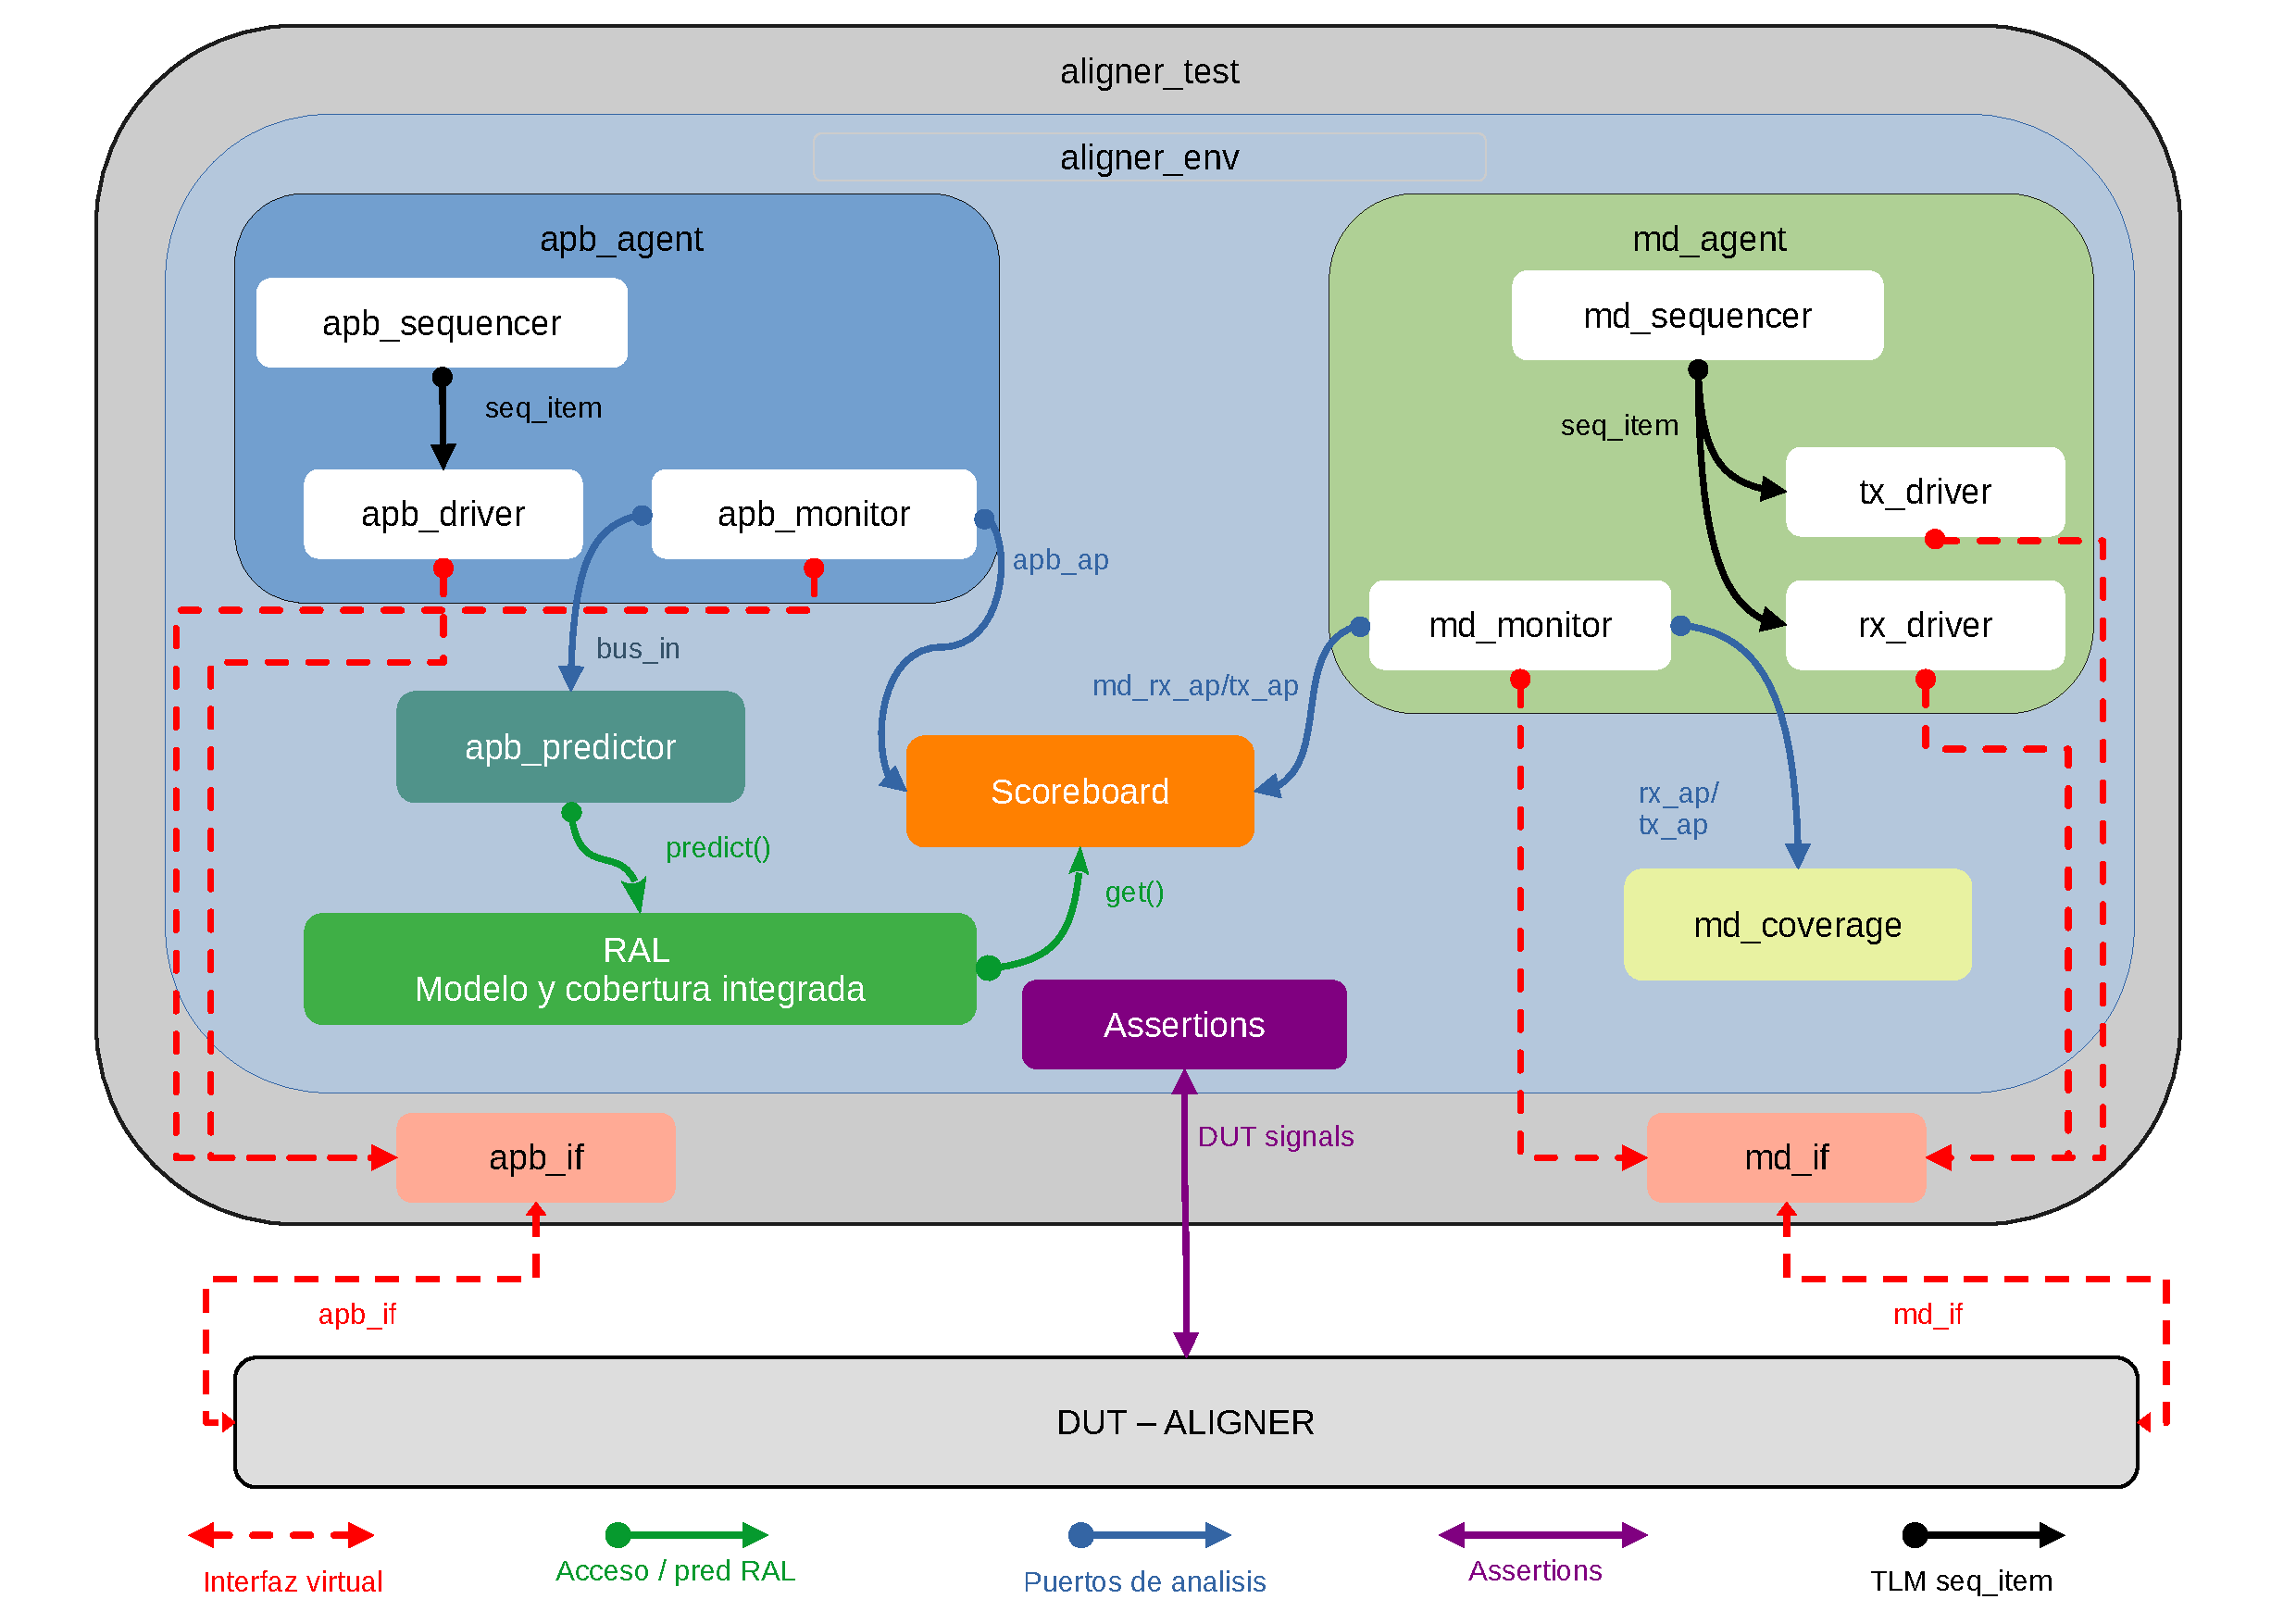
\includegraphics[width=0.82\textwidth]{diagrama_ambiente.pdf}
  \caption{Arquitectura del ambiente de verificación UVM. Los \textit{drivers}
  conducen el DUT a través de las interfaces virtuales; los \textit{monitors}
  publican las transacciones observadas hacia el \textit{scoreboard} por puertos
  de análisis. El RAL se conecta al secuenciador APB mediante el adaptador y se
  sincroniza con el \textit{scoreboard} por \texttt{predict()}/\texttt{get()}.}
  \label{fig:arquitectura}
\end{figure*}

\begin{table*}[t]
\caption{Plan de pruebas y su mapeo a plusargs sobre la prueba general \texttt{aligner\_test}}
\label{tab:testplan}
\centering
\footnotesize
\begin{tabular}{@{}p{0.4cm}p{4.3cm}p{8.5cm}p{2.6cm}@{}}
\toprule
\textbf{\#} & \textbf{Objetivo de verificación} & \textbf{Plusargs} & \textbf{Resultado esperado} \\
\midrule
1 & Configurar CTRL solo en bytes (size=1) & \texttt{+W\_CTRL\_SIZE1=100 +W\_CTRL\_SIZE2=0 +W\_CTRL\_SIZE4=0} & TX con size=1, cualquier offset. \\
2 & Configurar CTRL solo en words (size=4) & \texttt{+W\_CTRL\_SIZE4=100 +W\_CTRL\_SIZE1=0 +W\_CTRL\_SIZE2=0} & TX con size=4, offset=0. \\
3 & Solo offset base (0) & \texttt{+W\_CTRL\_OFF0=100 +W\_CTRL\_OFF1=0 +W\_CTRL\_OFF2=0 +W\_CTRL\_OFF3=0} & OFFSET=0 en todas las TX. \\
4 & Tráfico RX solo legal & \texttt{+W\_ILLEGAL=0 +NUM\_TRANSFERS=100} & \texttt{CNT\_DROP=0}, sin errores. \\
5 & Mezcla legal/ilegal & \texttt{+W\_ILLEGAL=30 +NUM\_TRANSFERS=100} & RX ilegales con \texttt{rx\_err=1}. \\
6 & Tráfico totalmente ilegal & \texttt{+W\_ILLEGAL=100 +NUM\_TRANSFERS=100} & Todas las RX descartadas. \\
7 & Contrapresión del consumidor TX & \texttt{+TX\_READY\_WEIGHT=20 +NUM\_TRANSFERS=100} & Acumulación en FIFO TX. \\
8 & Interrupción MAX\_DROP al saturar & \texttt{+W\_IRQEN\_MAX\_DROP=100 +W\_ILLEGAL=100 +NUM\_TRANSFERS=300} & \texttt{IRQ[4]=1}, \texttt{CNT\_DROP=255}. \\
9 & MAX\_DROP no dispara con $<255$ drops & \texttt{+W\_IRQEN\_MAX\_DROP=100 +W\_ILLEGAL=100 +NUM\_TRANSFERS=50} & \texttt{IRQ=0x00}. \\
10 & Limpieza de interrupción (W1C) & \texttt{+W\_IRQEN\_MAX\_DROP=100 +W\_IRQ\_CLR=100 +W\_ILLEGAL=100 +NUM\_TRANSFERS=300} & IRQ se limpia tras lectura. \\
11 & Reconfiguración dinámica de CTRL & \texttt{+N\_RECONFIG=3 +NUM\_TRANSFERS=200} & 4 bloques RX con CTRL distinto. \\
12 & Estrés combinado & \texttt{+NUM\_TRANSFERS=500 +W\_ILLEGAL=30 +TX\_READY\_WEIGHT=50 +N\_RECONFIG=3} & Sin errores de scoreboard. \\
\bottomrule
\end{tabular}
\end{table*}

\begin{table*}[t]
\caption{Casos de esquina considerados y su forma de alcance sobre la prueba general}
\label{tab:esquina}
\centering
\footnotesize
\begin{tabular}{@{}p{0.4cm}p{3.6cm}p{6.1cm}p{6.0cm}@{}}
\toprule
\textbf{\#} & \textbf{Caso de esquina} & \textbf{Cómo se alcanza (plusargs / mecanismo)} & \textbf{Comportamiento esperado} \\
\midrule
1  & Palabra completa (tamaño máximo)        & \texttt{+W\_CTRL\_SIZE4=100 +W\_CTRL\_OFF0=100} & TX de 4 bytes alineada, sin \textit{drops}. \\
2  & Offset máximo legal                     & \texttt{+W\_SIZE1=100 +W\_OFF3=100}            & RX legal con \texttt{rx\_err=0}. \\
3  & Halfword en offset par alto             & \texttt{+W\_SIZE2=100 +W\_OFF2=100}            & RX legal (\texttt{size=2, offset=2}). \\
4  & Tamaño nulo (\texttt{size=0})           & \texttt{+W\_ILLEGAL=100} (pool ilegal)         & \texttt{rx\_err=1}, transferencia descartada. \\
5  & Tamaño no potencia de 2 (\texttt{size=3})& \texttt{+W\_ILLEGAL=100} (pool ilegal)        & \texttt{rx\_err=1}, descartada. \\
6  & Halfword/word desalineados              & \texttt{+W\_ILLEGAL=100} (pool ilegal)         & \texttt{rx\_err=1} en \texttt{size=2} off impar y \texttt{size=4} off$\neq$0. \\
7  & \texttt{CNT\_DROP} bajo el umbral       & \texttt{+W\_ILLEGAL=100 +NUM\_TRANSFERS=254}   & \texttt{IRQ[4]=0}, \texttt{CNT\_DROP=254}. \\
8  & \texttt{CNT\_DROP} en el umbral exacto  & \texttt{+W\_ILLEGAL=100 +NUM\_TRANSFERS=255}   & \texttt{IRQ[4]=1}, \texttt{CNT\_DROP=0xFF}. \\
9  & \texttt{CNT\_DROP} saturado             & \texttt{+W\_ILLEGAL=100 +NUM\_TRANSFERS=300}   & \texttt{CNT\_DROP} se mantiene en \texttt{0xFF}. \\
10 & FIFO TX llena (back-pressure total)     & \texttt{+TX\_READY\_WEIGHT=0 +NUM\_TRANSFERS=100} & \texttt{TX\_LVL} al máximo, \texttt{TX\_FIFO\_FULL}. \\
11 & FIFO TX drenada por completo            & \texttt{+TX\_READY\_WEIGHT=100}                & \texttt{TX\_LVL=0} al final. \\
12 & Byte residual sin paquete completo      & Bytes acumulados no múltiplos del \texttt{SIZE} & Remanente en FIFO, \texttt{TX\_LVL}$>$0. \\
13 & Reconfiguración en caliente de CTRL     & \texttt{+N\_RECONFIG=3}                        & TX respetan la config vigente en cada bloque. \\
14 & Limpieza de interrupción (W1C)          & \texttt{+W\_IRQEN\_MAX\_DROP=100 +W\_IRQ\_CLR=100} & \texttt{IRQ} se limpia tras la lectura. \\
\bottomrule
\end{tabular}
\end{table*}

% =====================================================================
\begin{thebibliography}{00}
\bibitem{spear} C. Spear, \textit{SystemVerilog for Verification: A Guide to
Learning the Testbench Language Features}, 2nd ed. New York, NY: Springer, 2008.
\bibitem{uvm} Accellera, \textit{Universal Verification Methodology (UVM) 1.2
User's Guide}, 2015.
\bibitem{ieee1800} IEEE, \textit{IEEE Standard for SystemVerilog—Unified
Hardware Design, Specification, and Verification Language}, IEEE Std 1800-2017.
\bibitem{ieee18002} IEEE, \textit{IEEE Standard for Universal Verification
Methodology Language Reference Manual}, IEEE Std 1800.2-2020.
\bibitem{apb} ARM, \textit{AMBA APB Protocol Specification}, ARM IHI 0024.
\end{thebibliography}

\end{document}